\begin{frame}
	\frametitle{Fourier Reihe}
	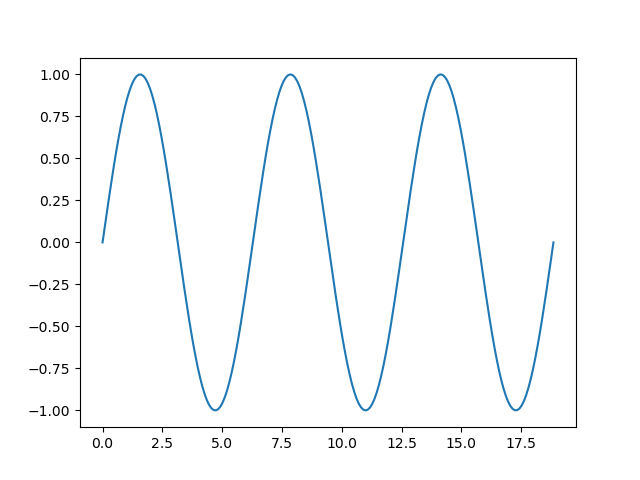
\includegraphics[width=200px]{images/00-rect-0.png}
\end{frame}

\begin{frame}
	\frametitle{Fourier Reihe}
	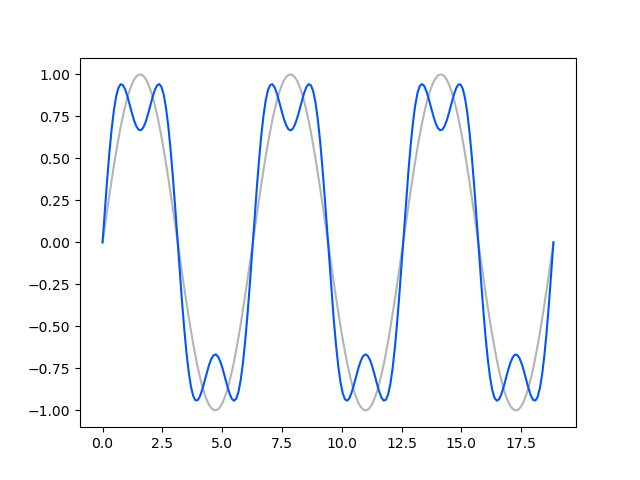
\includegraphics[width=200px]{images/00-rect-1.png}
\end{frame}

\begin{frame}
	\frametitle{Fourier Reihe}
	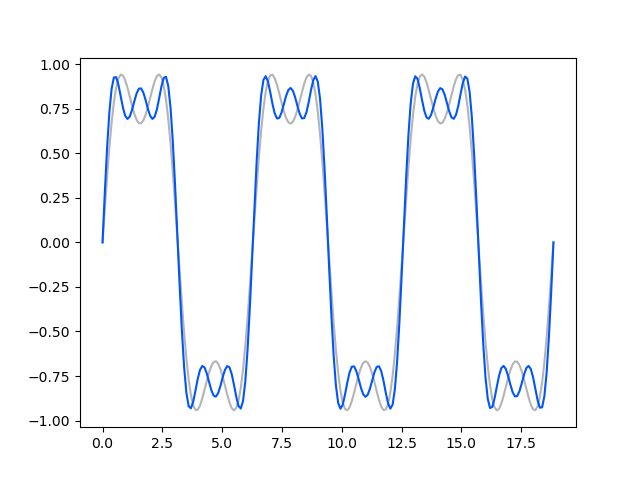
\includegraphics[width=200px]{images/00-rect-2.png}
\end{frame}

\begin{frame}
	\frametitle{Fourier Reihe}
	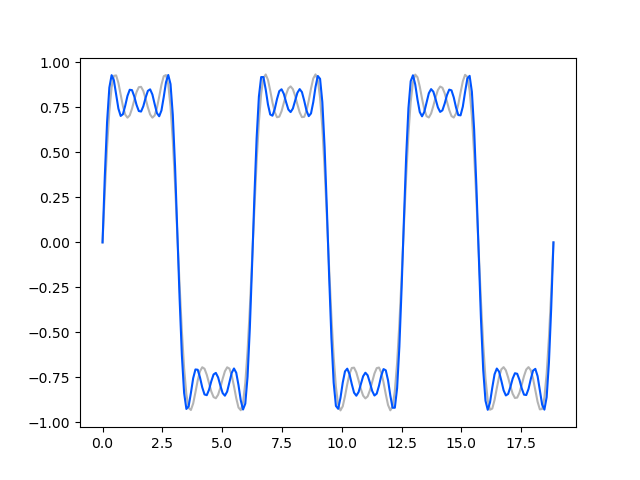
\includegraphics[width=200px]{images/00-rect-3.png}
\end{frame}

\begin{frame}
	\frametitle{Fourier Reihe}
	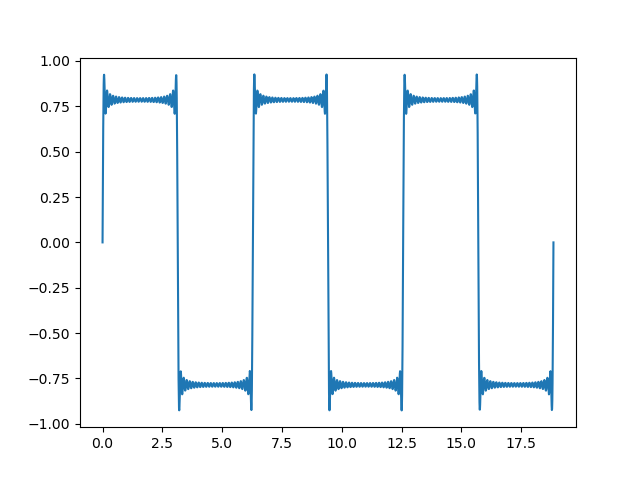
\includegraphics[width=200px]{images/00-rect-4.png}
\end{frame}

\begin{frame}
	\frametitle{Fourier Reihe}
	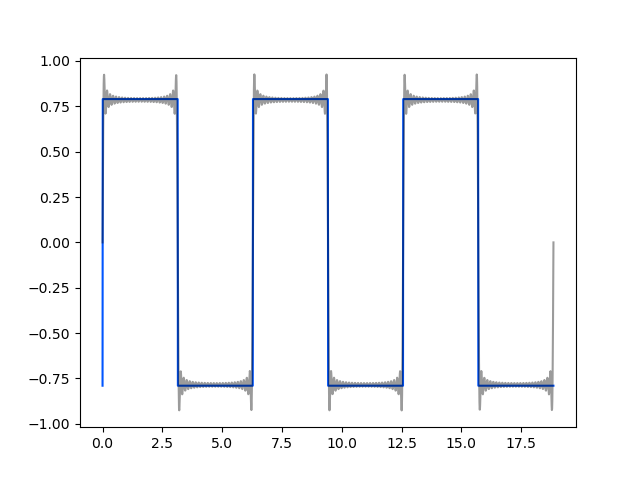
\includegraphics[width=200px]{images/00-rect-5.png}
\end{frame}

\begin{frame}
	\frametitle{Fourier Reihe}
	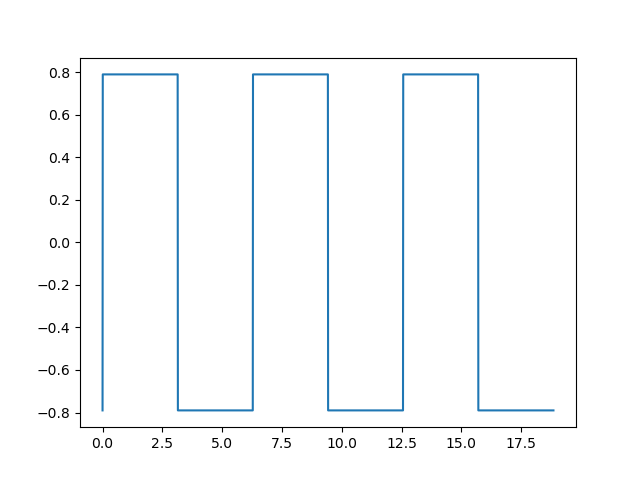
\includegraphics[width=200px]{images/00-rect-6.png}
	\begin{align}
		\sum_{k=1,3,5,\cdots}^{\infty}\frac{sin(kx)}{k}
	\end{align}
\end{frame}

\begin{frame}
	\frametitle{Fourier Reihe}
	\begin{itemize}
		\item Periodische Signale können durch Summen von Sinus- und Kosinuswellen approximiert werden
		\item Hierbei werden diese in eine Grundschwingung und Oberschwingungen mit ganzzahligen Vielfachen der Grundfrequenz aufgeteilt
		\item $f(t) = \displaystyle\frac{a_0}{2} + \displaystyle \sum_{k=1}^{\infty}\left[a_k cos(\omega_0 kt) + b_k sin(\omega_0 kt)\right]$
	\end{itemize}
\end{frame}

\begin{frame}
	\frametitle{Wieso Sinus und Kosinus}
	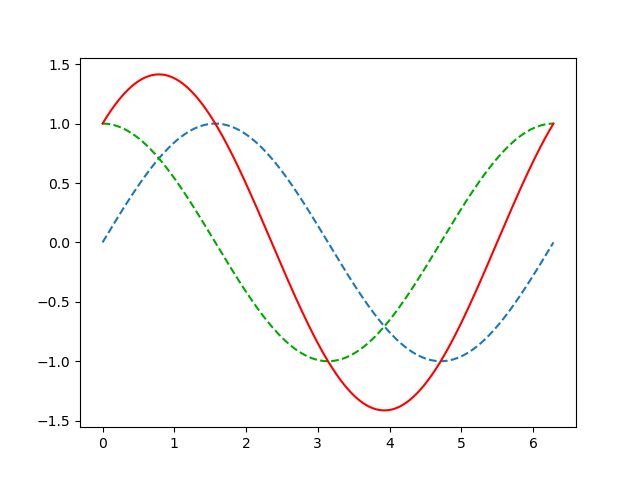
\includegraphics[width=200px]{images/00-sincos.png}
	\begin{itemize}
		\item Sinus ist punktsymmetrisch
		\item Kosinus ist achsensymmetrisch
		\item Phasenverschiebung durch Sinus-Kosinus Kombination
	\end{itemize}
\end{frame}

\begin{frame}
	\frametitle{Oberwellen}
	\begin{columns}
		\begin{column}{0.5\linewidth}
			\centering
			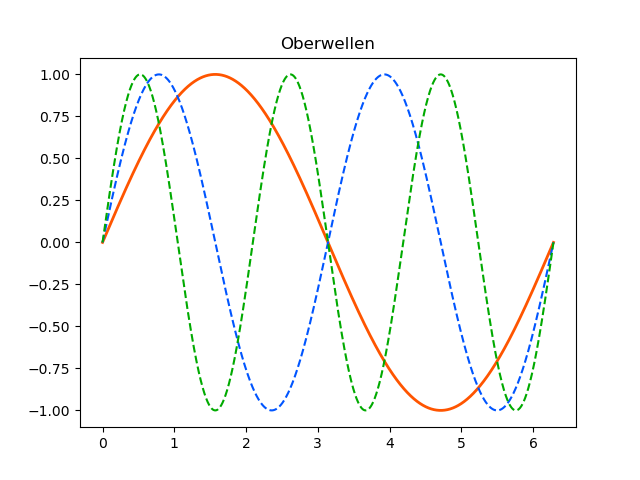
\includegraphics[width=170px]{images/00-oberwellen-0.png}
			Bei $\omega_k = n\,\omega_0$ wird die Grundfrequenz nicht beeinflusst.
		\end{column}
		\begin{column}{0.5\linewidth}
			\centering
			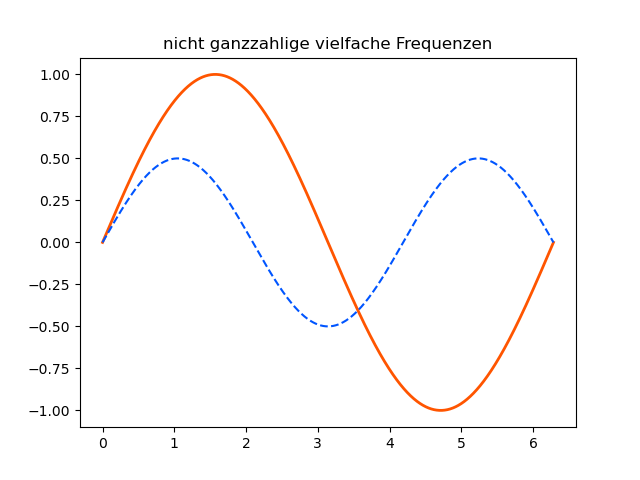
\includegraphics[width=170px]{images/00-oberwellen-1.png}
			Andere Frequenzen beeinflussen die Grundfrequenz der Schwingung
		\end{column}
	\end{columns}
\end{frame}

\begin{frame}
	\frametitle{Oberwellen}
	\begin{columns}
		\begin{column}{0.5\linewidth}
			\centering
			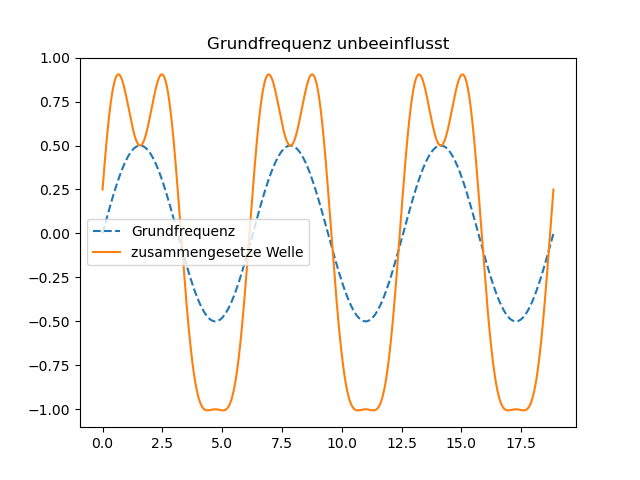
\includegraphics[width=170px]{images/00-oberwellen-zus-0.png}
			$sin(x) + \frac{cos(2x)}{4}+\frac{sin(3x)}{4}$
		\end{column}
		\begin{column}{0.5\linewidth}
			\centering
			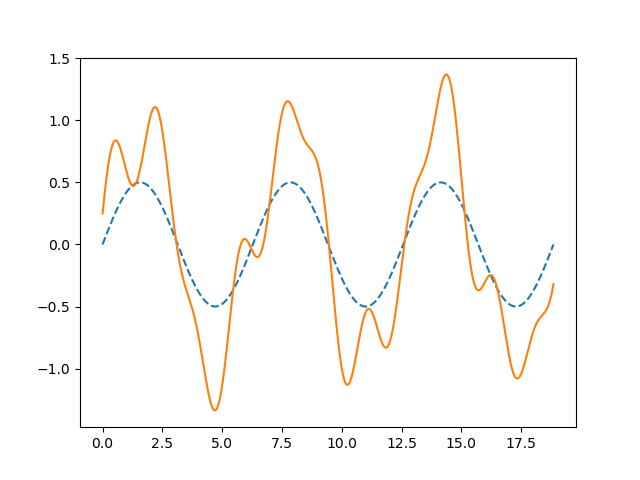
\includegraphics[width=170px]{images/00-oberwellen-zus-1.png}
			$sin(x) + \frac{cos(2.23x)}{4}+\frac{sin(3.56x)}{4}$
		\end{column}
	\end{columns}
\end{frame}

\begin{frame}
	\frametitle{Wie werden die Fourier Koeffizienten gewählt?}
\end{frame}

\begin{frame}
	\frametitle{Komplexe Darstellung der Fourierreihe}
	HIER MAREKS FOLIEN REIN !!!111!
\end{frame}

\begin{frame}
	\frametitle{Herleitung komplexe Darstellung}
	Komplexe Darstellung von Sinus und Kosinus:
	\begin{align*}
		cos(\varphi) &= \frac{e^{i\varphi}+e^{-i\varphi}}{2} \\
		sin(\varphi) &= \frac{e^{i\varphi}-e^{-i\varphi}}{2i}
	\end{align*}
\end{frame}
\begin{frame}
	\frametitle{Herleitung komplexe Darstellung}
	\begin{align*}
		f(t) &= \sum_{k=0}^{\infty}\left[a_k cos(kt) + b_k sin(kt)\right] \\
		&= \sum_{k=0}^{\infty}\left[a_k \frac{e^{ikt}+e^{-ikt}}{2} + b_k \frac{e^{ikt}-e^{-ikt}}{2i}\right] \\
		&= \sum_{k=0}^{\infty}\left[\frac{a_k}{2}e^{ikt} + \frac{a_k}{2}e^{-ikt} + \frac{b_k}{2i}e^{ikt} - \frac{b_k}{2i}e^{-ikt}\right] \\
		&= \sum_{k=0}^{\infty}\left[\frac{1}{2}\left(a_k-b_ki\right)e^{ikt} + \frac{1}{2}\left(a_k+b_ki\right)e^{-ikt}\right] \\
		&= \sum_{k=0}^{\infty}\left[\frac{1}{2}\left(a_k-b_ki\right)e^{ikt}\right] + \sum_{k=0}^{\infty}\left[\frac{1}{2}\left(a_k+b_ki\right)e^{-ikt}\right] \\
	\end{align*}
\end{frame}

\begin{frame}
	\frametitle{Herleitung komplexe Darstellung}
	\begin{align*}
		f(t) &= \sum_{k=0}^{\infty}\left[\frac{1}{2}\left(a_k-b_ki\right)e^{ikt}\right] + \sum_{k=0}^{\infty}\left[\frac{1}{2}\left(a_k+b_ki\right)e^{-ikt}\right] \\ \\
		Sei \,\,\, &\,c_k = \begin{cases}
			\,\,\displaystyle\frac{1}{2}(a_k - b_ki) \quad f\ddot{u}r\,\,\, k > 0 \\ \\
			\,\,\displaystyle\frac{1}{2}(a_k + b_ki) \quad f\ddot{u}r\,\,\, k \le 0 
		\end{cases} \\ \\
	f(t) &= \sum_{k=-\infty}^{\infty}c_k e^{ikt}
	\end{align*}
\end{frame}

\begin{frame}
	\frametitle{Berechnung der komplexen Koeffizienten}
	\begin{align*}
		\int_{0}^{T}f(t) e^{-imt}
		&= \int_{0}^{T} \left(\sum_{k=-\infty}^{\infty}c_k e^{ikt}\right) e^{-imt} dt \\
		&= \int_{0}^{T} \sum_{k=-\infty}^{\infty}c_k e^{i(k-m)t} dt \\
		&= \sum_{k=-\infty}^{\infty} \int_{0}^{T}c_k e^{i(k-m)t} dt \\
	\end{align*}
\end{frame}

\begin{frame}
	\frametitle{Berechnung der komplexen Koeffizienten}
	für $k = m$ gilt:
	\begin{align*}
		\int_{0}^{T}c_k e^{i(k-m)t} dt &= \int_{0}^{T}c_k dt = c_k T
	\end{align*}
	für $k \ne m$ gilt:
	\begin{align*}
		\int_{0}^{T}c_k e^{i(k-m)t} dt &= \left[\frac{c_k}{i(k-m)}e^{i(k-m)t}\right]_{0}^{T} \\
		&= \frac{c_k}{i(k-m)}e^{i(k-m)T} - \frac{c_k}{i(k-m)} \\
		&= \frac{c_k}{i(k-m)} - \frac{c_k}{i(k-m)} = 0
	\end{align*}
\end{frame}

\begin{frame}
	\frametitle{Berechnung der komplexen Koeffizienten}
	\begin{align*}
		\sum_{k=-\infty}^{\infty}& \int_{0}^{T}c_k e^{i(k-m)t} dt = c_mT \\
		\to \quad & c_m = \frac{1}{T} \int_{0}^{T}f(t) e^{-imt}
	\end{align*}
\end{frame}